\section{Capítulo 2 -- Design RESTful e métodos HTTP}

No Capítulo 1, o REST apareceu como o estilo que organiza a API em torno de recursos e usa os métodos do HTTP. Mas dizer que uma API ``é REST'' não basta: duas APIs REST podem ser fáceis ou difíceis de usar dependendo de como foram projetadas. Neste capítulo você vai conhecer as regras do estilo REST, aprender a escolher boas URLs, entender o significado preciso de cada método HTTP, inclusive os conceitos de método seguro e idempotente, e ver as convenções de filtros, paginação e versionamento. No final, vai projetar no papel a API completa do TaskFlow, antes de escrever qualquer código.

\subsection{2.1 Recursos e representações}

Em REST, tudo gira em torno de \textbf{recursos}: as ``coisas'' que o sistema guarda e que fazem sentido para quem usa a API. No TaskFlow, os recursos são os usuários e as tarefas. Em uma loja, seriam produtos, clientes e pedidos.

Cada recurso tem um identificador único, a sua \textbf{URI} (\textit{Uniform Resource Identifier}), como \texttt{/api/tasks/42}. A URI é o ``endereço'' do recurso, e não muda conforme a ação: buscar, alterar e excluir a tarefa 42 usam todas a mesma URI, com métodos diferentes.

O cliente nunca recebe o recurso em si, que está guardado no banco de dados, e sim uma \textbf{representação} dele: um retrato em algum formato, quase sempre JSON. O mesmo recurso pode ter várias representações. O cliente diz qual prefere com o cabeçalho \texttt{Accept}, e o servidor informa qual enviou com o \texttt{Content-Type}:

\begin{codigo}
\begin{Verbatim}[breaklines=true, breaksymbolleft={}, fontsize=\footnotesize]
GET /api/tasks/42 HTTP/1.1
Accept: application/json

HTTP/1.1 200 OK
Content-Type: application/json

{"id": 42, "title": "Estudar REST", "status": "PENDING"}
\end{Verbatim}
\end{codigo}

Essa escolha do formato pelos cabeçalhos se chama \textbf{negociação de conteúdo} e volta no Capítulo 5, com JSON e XML.

\subsection{2.2 As restrições do REST}

Roy Fielding definiu o REST como um conjunto de \textbf{restrições}: regras que, quando seguidas, dão ao sistema escalabilidade, simplicidade e independência entre as partes. Uma API é RESTful quando respeita essas regras:

\begin{center}
\begin{tabular}{@{}P{0.28\linewidth}P{0.62\linewidth}@{}}
\toprule
\rowcolor{headergray}
\tblheader{Restrição} & \tblheader{O que significa} \\
\midrule
cliente-servidor & interface e dados ficam separados; o site, o aplicativo e o servidor evoluem de forma independente \\
\rowcolor{rowgray} sem estado & cada requisição traz tudo o que o servidor precisa; ele não guarda sessão entre uma e outra \\
\textit{cache} & a resposta diz se pode ser guardada e reaproveitada, o que poupa requisições \\
\rowcolor{rowgray} interface uniforme & recursos identificados por URIs, manipulados por representações, com mensagens que se explicam sozinhas \\
sistema em camadas & o cliente não sabe se fala direto com o servidor ou com intermediários, como um balanceador de carga ou uma CDN \\
\rowcolor{rowgray} código sob demanda (opcional) & o servidor pode enviar código para o cliente executar, como um \textit{script} \\
\bottomrule
\end{tabular}
\end{center}

A restrição \textbf{sem estado} é a que mais influencia o projeto. Como o servidor não guarda nada entre as requisições, qualquer servidor de um grupo pode atender qualquer requisição. É isso que permite colocar dez cópias da API atrás de um balanceador de carga quando o número de usuários cresce. O preço é que o cliente precisa mandar, a cada requisição, a sua identificação, normalmente um \textit{token}.

\subsection{2.3 Boas URLs}

A URL é a primeira coisa que o desenvolvedor vê da sua API, e um bom padrão torna a API previsível: quem aprendeu a listar tarefas consegue adivinhar como listar usuários. As convenções mais aceitas são estas:

\begin{itemize}
  \item \textbf{Use substantivos, nunca verbos.} A ação já está no método HTTP. \texttt{POST /tasks}, e não \texttt{POST /criarTarefa}.
  \item \textbf{Use o plural para coleções.} \texttt{/tasks} é a coleção; \texttt{/tasks/42} é um item dela. O mesmo nome serve aos dois casos.
  \item \textbf{Mostre a hierarquia quando ela existe.} As tarefas do usuário 7 ficam em \texttt{/users/7/tasks}. Evite passar de dois níveis: \texttt{/users/7/tasks/42/comments/3} já é difícil de manter.
  \item \textbf{Use letras minúsculas e hífens.} \texttt{/task-categories}, e não \texttt{/TaskCategories} nem \texttt{/task\_categories}. Partes da URL podem diferenciar maiúsculas de minúsculas, o que confunde.
  \item \textbf{Filtros vão na \textit{query string}.} \texttt{/tasks?status=DONE}, e não \texttt{/tasks/done}: a tarefa concluída continua sendo uma tarefa.
  \item \textbf{Não exponha detalhes de implementação.} Nada de \texttt{/tasks.php} ou \texttt{/api/tabela\_tarefas}. Se a tecnologia mudar, a URL continua a mesma.
\end{itemize}

\begin{center}
\begin{tabular}{@{}P{0.45\linewidth}P{0.45\linewidth}@{}}
\toprule
\rowcolor{headergray}
\tblheader{Evite} & \tblheader{Prefira} \\
\midrule
\texttt{GET /getTasks} & \texttt{GET /tasks} \\
\rowcolor{rowgray} \texttt{POST /tasks/create} & \texttt{POST /tasks} \\
\texttt{GET /task/42} & \texttt{GET /tasks/42} \\
\rowcolor{rowgray} \texttt{POST /tasks/42/delete} & \texttt{DELETE /tasks/42} \\
\texttt{GET /tasks/pendentes} & \texttt{GET /tasks?status=PENDING} \\
\rowcolor{rowgray} \texttt{GET /tasksDoUsuario?id=7} & \texttt{GET /users/7/tasks} \\
\bottomrule
\end{tabular}
\end{center}

Há casos em que uma ação não se encaixa bem em criar, ler, alterar ou excluir, como ``reenviar o e-mail de confirmação''. A saída usual é tratar a ação como um sub-recurso e usar \texttt{POST}: \texttt{POST /users/7/confirmation-email}. Use isso com moderação; na maioria das vezes, a ação pode ser expressa como alteração de um campo, como \texttt{PATCH /tasks/42} com \texttt{\{"status": "DONE"\}} em vez de \texttt{POST /tasks/42/concluir}.

\subsection{2.4 Os métodos HTTP}

O método diz \textbf{o que} o cliente quer fazer com o recurso indicado pela URL. Cada método tem um significado definido pela especificação do HTTP (a RFC 9110), e respeitá-lo é o que permite a navegadores, \textit{caches} e bibliotecas tratarem a sua API corretamente.

\begin{center}
\begin{tabular}{@{}P{0.15\linewidth}P{0.4\linewidth}P{0.11\linewidth}P{0.11\linewidth}P{0.11\linewidth}@{}}
\toprule
\rowcolor{headergray}
\tblheader{Método} & \tblheader{Uso} & \tblheader{Corpo} & \tblheader{Seguro} & \tblheader{Idem\-po\-ten\-te} \\
\midrule
\texttt{GET} & buscar um recurso ou uma coleção & não & sim & sim \\
\rowcolor{rowgray} \texttt{POST} & criar um recurso em uma coleção & sim & não & não \\
\texttt{PUT} & substituir o recurso inteiro & sim & não & sim \\
\rowcolor{rowgray} \texttt{PATCH} & alterar parte do recurso & sim & não & não* \\
\texttt{DELETE} & excluir o recurso & não & não & sim \\
\rowcolor{rowgray} \texttt{HEAD} & como o GET, mas só os cabeçalhos & não & sim & sim \\
\texttt{OPTIONS} & perguntar quais métodos a URL aceita & não & sim & sim \\
\bottomrule
\end{tabular}
\end{center}

{\footnotesize * O PATCH pode ser idempotente, dependendo de como a alteração é descrita (Seção 2.6).}

O \texttt{HEAD} serve, por exemplo, para saber o tamanho de um arquivo pelo cabeçalho \texttt{Content-Length} sem baixá-lo. O \texttt{OPTIONS} é usado automaticamente pelo navegador antes de certas requisições entre domínios diferentes, no mecanismo chamado CORS, estudado no Capítulo 12.

\subsection{2.5 Métodos seguros e idempotentes}

Duas propriedades da tabela anterior merecem atenção, porque são cobradas com frequência e evitam erros graves.

Um método é \textbf{seguro} quando não altera nada no servidor: ele só lê. \texttt{GET}, \texttt{HEAD} e \texttt{OPTIONS} são seguros. Por isso, navegadores e robôs de busca seguem links (que fazem \texttt{GET}) livremente, e ferramentas de \textit{cache} guardam as respostas. Uma API que exclui algo em um \texttt{GET}, como \texttt{GET /tasks/42/delete}, corre o risco de ver os dados sumirem quando um robô ou uma pré-visualização de link visitar a URL.

Um método é \textbf{idempotente} quando repetir a mesma requisição várias vezes deixa o servidor no mesmo estado que fazê-la uma vez só. Pense em um elevador: apertar o botão do 5º andar uma ou dez vezes leva ao mesmo lugar.

\begin{itemize}
  \item \texttt{DELETE /tasks/42} é idempotente: depois da primeira vez, a tarefa já não existe, e as repetições não mudam nada. A resposta pode mudar (a segunda recebe \texttt{404}), mas o \textbf{estado} do servidor é o mesmo.
  \item \texttt{PUT /tasks/42} com a tarefa completa é idempotente: gravar os mesmos dados de novo dá no mesmo.
  \item \texttt{POST /tasks} \textbf{não} é idempotente: cada repetição cria uma tarefa nova.
\end{itemize}

Isso importa na prática por causa das falhas de rede. Se o cliente envia uma requisição e a conexão cai antes da resposta, ele não sabe se o servidor a recebeu. Com um método idempotente, basta repetir. Com um \texttt{POST}, repetir pode criar um pedido em dobro, e é por isso que sites de compra pedem para você não apertar o botão ``Pagar'' duas vezes. APIs de pagamento resolvem o problema com uma \textbf{chave de idempotência}: o cliente gera um código único e o envia em um cabeçalho, como \texttt{Idempotency-Key}; se o servidor já processou aquele código, devolve o resultado anterior em vez de cobrar de novo.

\subsection{2.6 PUT ou PATCH?}

Os dois alteram um recurso existente, mas de formas diferentes. O \texttt{PUT} \textbf{substitui} o recurso inteiro pela representação enviada; o \texttt{PATCH} aplica uma \textbf{alteração parcial}. Considere a tarefa 42:

\begin{codigo}
\begin{Verbatim}[breaklines=true, breaksymbolleft={}, fontsize=\footnotesize]
{"id": 42, "title": "Estudar REST",
 "status": "PENDING", "priority": "HIGH"}
\end{Verbatim}
\end{codigo}

Para marcá-la como concluída, o \texttt{PATCH} envia só o que muda:

\begin{codigo}
\begin{Verbatim}[breaklines=true, breaksymbolleft={}, fontsize=\footnotesize]
PATCH /api/tasks/42
{"status": "DONE"}
\end{Verbatim}
\end{codigo}

Com \texttt{PUT}, é preciso enviar a tarefa completa. Se o cliente mandar só \texttt{\{"status": "DONE"\}}, um servidor que segue a regra à risca entende que o título e a prioridade foram retirados:

\begin{codigo}
\begin{Verbatim}[breaklines=true, breaksymbolleft={}, fontsize=\footnotesize]
PUT /api/tasks/42
{"title": "Estudar REST", "status": "DONE", "priority": "HIGH"}
\end{Verbatim}
\end{codigo}

Na prática, o \texttt{PATCH} é o mais usado para edições, porque os formulários costumam alterar poucos campos e a requisição fica menor. Um \texttt{PATCH} como o acima, que define valores, é idempotente. Já um \texttt{PATCH} que descreve uma operação relativa, como ``some 1 ao contador de visualizações'', não é: cada repetição soma de novo. Por isso a especificação não garante a idempotência do \texttt{PATCH}. A API do TaskFlow usa \texttt{PATCH} para editar tarefas.

\subsection{2.7 Os códigos de status mais usados}

O código de status resume o resultado em três dígitos, e o primeiro indica a família:

\begin{center}
\begin{tabular}{@{}P{0.13\linewidth}P{0.77\linewidth}@{}}
\toprule
\rowcolor{headergray}
\tblheader{Família} & \tblheader{Significado} \\
\midrule
\texttt{1xx} & informação: a requisição foi recebida e continua em processamento (raro em APIs) \\
\rowcolor{rowgray} \texttt{2xx} & sucesso \\
\texttt{3xx} & redirecionamento: o recurso está em outro lugar \\
\rowcolor{rowgray} \texttt{4xx} & erro do cliente: a requisição tem algum problema \\
\texttt{5xx} & erro do servidor: a requisição estava certa, mas o servidor falhou \\
\bottomrule
\end{tabular}
\end{center}

A distinção entre \texttt{4xx} e \texttt{5xx} é importante: com \texttt{4xx}, o cliente precisa corrigir algo antes de tentar de novo; com \texttt{5xx}, a mesma requisição pode funcionar mais tarde. Os códigos que aparecem em quase toda API são estes, e o Capítulo 8 trata de como escolher e montar as respostas de erro:

\begin{center}
\begin{tabular}{@{}P{0.25\linewidth}P{0.65\linewidth}@{}}
\toprule
\rowcolor{headergray}
\tblheader{Código} & \tblheader{Quando usar} \\
\midrule
\texttt{200 OK} & sucesso com corpo na resposta: GET, PUT, PATCH \\
\rowcolor{rowgray} \texttt{201 Created} & POST que criou um recurso; envie o cabeçalho \texttt{Location} com a URI dele \\
\texttt{204 No Content} & sucesso sem corpo, típico do DELETE \\
\rowcolor{rowgray} \texttt{400 Bad Request} & dados malformados ou inválidos \\
\texttt{401 Unauthorized} & falta autenticação, ou o \textit{token} é inválido \\
\rowcolor{rowgray} \texttt{403 Forbidden} & autenticado, mas sem permissão para aquele recurso \\
\texttt{404 Not Found} & o recurso não existe \\
\rowcolor{rowgray} \texttt{405 Method Not Allowed} & a URL existe, mas não aceita aquele método \\
\texttt{409 Conflict} & conflito com o estado atual, como um e-mail já cadastrado \\
\rowcolor{rowgray} \texttt{500 Internal Server Error} & falha inesperada no servidor \\
\bottomrule
\end{tabular}
\end{center}

\subsection{2.8 Filtros, ordenação e paginação}

Uma coleção pode ter milhares de itens, e devolver tudo de uma vez deixa a API lenta e a resposta enorme. As operações sobre coleções usam a \textit{query string}, com nomes que sigam sempre o mesmo padrão:

\begin{codigo}
\begin{Verbatim}[breaklines=true, breaksymbolleft={}, fontsize=\footnotesize]
GET /api/tasks?status=PENDING&priority=HIGH
GET /api/tasks?search=relatorio
GET /api/tasks?sort=dueDate
GET /api/tasks?sort=-createdAt
GET /api/tasks?page=2&limit=10
\end{Verbatim}
\end{codigo}

Os filtros usam o nome do próprio campo. A busca por texto costuma usar \texttt{search} ou \texttt{q}. Na ordenação, uma convenção comum é o sinal de menos indicar a ordem decrescente: \texttt{-createdAt} lista as mais recentes primeiro. Na \textbf{paginação}, \texttt{page} indica a página e \texttt{limit} quantos itens vêm em cada uma. A resposta deve informar ao cliente quanto falta, para que ele saiba se mostra o botão ``próxima página'':

\begin{codigo}
\begin{Verbatim}[breaklines=true, breaksymbolleft={}, fontsize=\footnotesize]
{
  "data": [
    {"id": 11, "title": "Revisar capítulo 1"},
    {"id": 12, "title": "Ler sobre PATCH"}
  ],
  "meta": {"page": 2, "limit": 10, "total": 37, "totalPages": 4}
}
\end{Verbatim}
\end{codigo}

Os dados ficam em \texttt{data} e as informações da paginação em \texttt{meta}. Esse ``envelope'' é uma convenção, e não uma regra do REST, mas usar sempre o mesmo formato facilita a vida de quem consome a API. Defina também um \texttt{limit} máximo, como 100: sem ele, um cliente pode pedir \texttt{limit=1000000} e sobrecarregar o servidor.

A paginação por número de página é simples, mas tem um defeito: se uma tarefa nova é criada enquanto o usuário navega, os itens ``escorregam'' e um deles aparece em duas páginas. APIs com muito movimento, como as de redes sociais, usam a paginação por \textbf{cursor}: a resposta traz um código que aponta para o último item visto, e a próxima página começa depois dele (\texttt{?cursor=abc123}).

\subsection{2.9 Versionamento}

Uma API publicada tem clientes que dependem dela, e mudar o contrato pode quebrá-los. Mudanças que \textbf{não quebram} os clientes, como acrescentar um campo novo na resposta ou um \textit{endpoint} novo, podem ser feitas a qualquer momento. Mudanças que \textbf{quebram}, como renomear ou remover um campo, mudar o tipo de um valor ou tornar obrigatório um campo que era opcional, exigem uma nova \textbf{versão} da API.

A forma mais comum e mais visível é colocar a versão na URL:

\begin{codigo}
\begin{Verbatim}[breaklines=true, breaksymbolleft={}, fontsize=\footnotesize]
GET /api/v1/tasks
GET /api/v2/tasks
\end{Verbatim}
\end{codigo}

Outra opção é indicar a versão em um cabeçalho, deixando as URLs limpas. Qualquer que seja a escolha, a versão antiga deve continuar funcionando por um tempo, com aviso aos clientes, até ser desativada. A API do TaskFlow é pequena e tem um único cliente no início, então começa sem versão; se um dia precisar de uma segunda versão, ela nasce em \texttt{/api/v2}.

\subsection{2.10 HATEOAS e o modelo de maturidade}

A última parte da restrição de interface uniforme tem um nome comprido: \textbf{HATEOAS} (\textit{Hypermedia as the Engine of Application State}). A ideia é que a resposta traga \textbf{links} para as ações possíveis, como uma página web traz links para as próximas páginas. O cliente descobre o que pode fazer navegando, sem precisar conhecer todas as URLs de antemão:

\begin{codigo}
\begin{Verbatim}[breaklines=true, breaksymbolleft={}, fontsize=\footnotesize]
{
  "id": 42,
  "title": "Estudar REST",
  "status": "PENDING",
  "_links": {
    "self":     {"href": "/api/tasks/42"},
    "complete": {"href": "/api/tasks/42", "method": "PATCH"},
    "delete":   {"href": "/api/tasks/42", "method": "DELETE"}
  }
}
\end{Verbatim}
\end{codigo}

Leonard Richardson propôs um modelo que classifica as APIs em quatro níveis, conforme o quanto aproveitam as ideias do REST:

\begin{center}
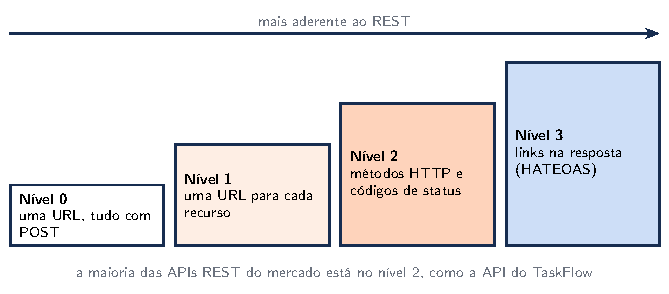
\includegraphics[width=0.95\linewidth,keepaspectratio]{imagens/capitulo-02_maturidade.pdf}
\end{center}

No \textbf{nível 0}, a API usa o HTTP só como transporte: uma URL e tudo com \texttt{POST}, como no SOAP. No \textbf{nível 1}, cada recurso tem a sua URL. No \textbf{nível 2}, os métodos e os códigos de status são usados com o seu significado. O \textbf{nível 3} acrescenta os links. A grande maioria das APIs chamadas de REST está no nível 2, que já traz quase todos os benefícios práticos, e é o nível da API do TaskFlow.

\subsection{2.11 Projetando a API do TaskFlow}

Antes de escrever código, uma boa prática é desenhar a API: listar os recursos, os \textit{endpoints}, o que cada um recebe e o que devolve. Esse desenho serve de contrato entre quem faz o servidor e quem faz o cliente, que podem trabalhar ao mesmo tempo.

O TaskFlow tem dois recursos. O \textbf{usuário} tem nome, e-mail e senha. A \textbf{tarefa} tem título, descrição opcional, situação (\texttt{PENDING}, \texttt{IN\_PROGRESS} ou \texttt{DONE}), prioridade (\texttt{LOW}, \texttt{MEDIUM} ou \texttt{HIGH}) e data de vencimento opcional, e pertence a um usuário. Cada pessoa só enxerga as próprias tarefas, então a URL não precisa trazer o usuário: o servidor descobre quem é pelo \textit{token}. Por isso a API usa \texttt{/api/tasks}, e não \texttt{/api/users/7/tasks}.

\begin{center}
\begin{tabular}{@{}P{0.27\linewidth}P{0.36\linewidth}P{0.27\linewidth}@{}}
\toprule
\rowcolor{headergray}
\tblheader{Endpoint} & \tblheader{Recebe} & \tblheader{Sucesso} \\
\midrule
\texttt{POST /api/auth/register} & nome, e-mail e senha & \texttt{201} e o usuário, sem a senha \\
\rowcolor{rowgray} \texttt{POST /api/auth/login} & e-mail e senha & \texttt{200} e o \textit{token} \\
\texttt{GET /api/tasks} & filtros: \texttt{status}, \texttt{priority}, \texttt{search}, \texttt{sort}, \texttt{page}, \texttt{limit} & \texttt{200}, \texttt{data} e \texttt{meta} \\
\rowcolor{rowgray} \texttt{POST /api/tasks} & título e, opcionalmente, os demais campos & \texttt{201}, a tarefa e \texttt{Location} \\
\texttt{GET /api/tasks/:id} & -- & \texttt{200} e a tarefa \\
\rowcolor{rowgray} \texttt{PATCH /api/tasks/:id} & os campos que mudam & \texttt{200} e a tarefa atualizada \\
\texttt{DELETE /api/tasks/:id} & -- & \texttt{204}, sem corpo \\
\bottomrule
\end{tabular}
\end{center}

Os erros também fazem parte do contrato. Todo \textit{endpoint} de tarefas responde \texttt{401} sem um \textit{token} válido; os que recebem dados respondem \texttt{400} quando eles são inválidos; os que usam \texttt{:id} respondem \texttt{404} quando a tarefa não existe \textbf{ou pertence a outra pessoa}. Responder \texttt{404}, e não \texttt{403}, no segundo caso evita revelar que existe uma tarefa com aquele número. O cadastro responde \texttt{409} quando o e-mail já está em uso. Um exemplo completo de criação:

\begin{codigo}
\begin{Verbatim}[breaklines=true, breaksymbolleft={}, fontsize=\footnotesize]
POST /api/tasks HTTP/1.1
Authorization: Bearer eyJhbGciOi...
Content-Type: application/json

{"title": "Entregar o trabalho", "priority": "HIGH",
 "dueDate": "2026-12-01"}
\end{Verbatim}
\end{codigo}

\begin{codigo}
\begin{Verbatim}[breaklines=true, breaksymbolleft={}, fontsize=\footnotesize]
HTTP/1.1 201 Created
Location: /api/tasks/cm3x9k2a0001
Content-Type: application/json

{
  "id": "cm3x9k2a0001",
  "title": "Entregar o trabalho",
  "description": null,
  "status": "PENDING",
  "priority": "HIGH",
  "dueDate": "2026-12-01T00:00:00.000Z",
  "createdAt": "2026-10-16T14:05:12.000Z"
}
\end{Verbatim}
\end{codigo}

Repare em três detalhes. O servidor preencheu sozinho os campos que o cliente não enviou: \texttt{status} começou como \texttt{PENDING}, e \texttt{description} veio como \texttt{null}. O identificador não é um número sequencial, e sim um texto aleatório (um \textit{cuid}), gerado pelo banco no Capítulo 3; isso impede que alguém adivinhe quantas tarefas existem ou tente os números em sequência. E as datas vêm no formato ISO 8601, com o fuso UTC indicado pelo \texttt{Z}, assunto do Capítulo 5.

\subsection{Erros Comuns}

\begin{itemize}
  \item \textbf{Verbos na URL.} \texttt{/getTasks} ou \texttt{/deleteTask/42} repetem o que o método já diz. Use substantivos e deixe a ação para o método.
  \item \textbf{Alterar dados com GET.} O GET deve ser seguro. Robôs, pré-visualizações de links e \textit{caches} fazem GET sem pedir licença.
  \item \textbf{Usar POST para tudo.} A API funciona, mas perde o significado dos métodos, a idempotência e o \textit{cache}: é o nível 0 de maturidade.
  \item \textbf{Mandar só parte dos campos em um PUT.} O PUT substitui o recurso inteiro. Para alterar só alguns campos, use PATCH.
  \item \textbf{Responder 200 para tudo, inclusive erros.} O cliente precisa ler o corpo para saber se deu certo. Use os códigos de status com o seu significado.
  \item \textbf{Confundir 401 e 403.} 401: ``não sei quem é você''. 403: ``sei quem é você, mas você não pode''.
  \item \textbf{Devolver a coleção inteira sem paginação.} Funciona com dez itens e derruba o servidor com cem mil. Defina um limite máximo.
  \item \textbf{Mudar o formato da resposta sem nova versão.} Renomear um campo quebra todos os clientes que dependem dele.
\end{itemize}
